\subsection{The Topic/Problem}

This section of the proposal targets a lack of high-order accurate and
provably stable interface conditions between structured and unstructured
meshes for computational fluid dynamic simulations. In particular, our aim
is to create a provably stable and accurate interface between summation-by-parts
finite difference discretizations (structured) and discontinuous Galerkin
methods (unstructured).  Achieving this would provide an option to create localized
areas of unstructured meshing (with superior flexibility for discretizing complex
boundaries/geometries) in existing simulations, providing an alternative to
overset curvilinear meshes.


\begin{figure}
\centering
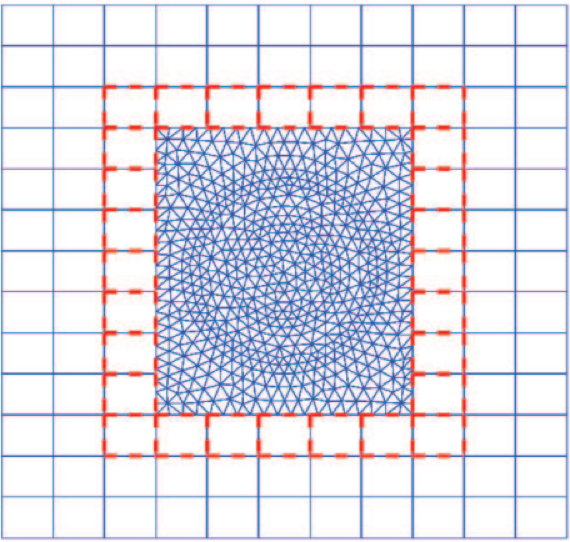
\includegraphics[width=0.3\linewidth,trim=4 4 4 4,clip]{figures/nonconforming_sample_1.png}
\caption{An example of a discretization for which we hope to achieve a stable and accurate nonconforming interface.
         Image credit: \emph{A Hybrid FETD-FDTD Method with Nonconforming Meshes}, B. Zhu, J. Chen, W. Zhong, Q. Liu.
         Commun. Computational Physics, Vol. 9, No. 3, pp. 828-842. March 2011.}
\label{fig:nonconforming_1}
\end{figure}

%===========================================================================
\subsection{Goals and Bounds}
(insert text here)

%===========================================================================
\subsection{The Plan}
(Insert text here)

%===========================================================================
\subsection{Impact}
(Insert text here)

%===========================================================================
\subsection{Risk Mitigation}
(Insert text here)

%===========================================================================
\subsection{Current Status}
(Insert text here)

%===========================================================================
